%% ============================================================
%%  A Click is All You Need — Demo Presentation
%%  研究生PPT汇报解救器 示例幻灯片
%%  Engine: XeLaTeX  |  Compile twice
%% ============================================================
\documentclass[aspectratio=169,10pt]{beamer}

%% ============================================================
%%  A Click is All You Need · 用户配置区 User Configuration
%%  ──────────────────────────────────────────────────────────
%%  只需编辑此文件即可调整字体、配色、页脚
%%  Edit ONLY this file to change fonts, colors, and footer.
%%  ──────────────────────────────────────────────────────────
%%  设计灵感 / Design Inspiration:
%%    - Pedro H.C. Sant'Anna (Vanderbilt / Microsoft Research)
%%      Beamer color palette and slide rhythm conventions
%%    - Isaiah Andrews (Harvard) — content density and
%%      information hierarchy in academic presentations
%%    - Till Tantau et al. — Beamer User Guide framework
%% ============================================================

%% ── 中文字体 / CJK Font ──────────────────────────────────────
%% macOS (system default):  Kaiti SC
%% Windows (system):        KaiTi
%% Linux (install first):   AR PL UKai CN
%%   sudo apt install fonts-arphic-ukai
\newcommand{\cjkfont}{Kaiti SC}

%% ── 英文字体 / Latin Font ────────────────────────────────────
%% Academic standard:  Times New Roman
%% Modern sans-serif:  Helvetica Neue
%% Elegant serif:      Palatino
\newcommand{\latinfont}{Times New Roman}

%% ── 主色系 / Primary Color Presets ──────────────────────────
%% Preset A — Deep Blue (Academic, default)
\definecolor{deepblue}{RGB}{0,52,102}

%% Preset B — Forest Green (Fresh) — uncomment to use:
%% \definecolor{deepblue}{RGB}{0,80,60}

%% Preset C — Academic Purple (Modern) — uncomment to use:
%% \definecolor{deepblue}{RGB}{60,20,100}

%% Custom: replace RGB values above with your preferred color.

%% ── 辅助色 / Supporting Colors ───────────────────────────────
%% Accent (brick red — alertblocks, highlights)
\definecolor{accent}{RGB}{196,72,49}

%% Light background (cover/ending frames)
\definecolor{lightbg}{RGB}{240,245,252}

%% Gold (key quotes, \textcolor{gold}{...})
\definecolor{gold}{RGB}{180,140,40}

%% Dark gray (body text fallback)
\definecolor{darkgray}{RGB}{60,60,60}

%% ── 页脚文字 / Footer Text ───────────────────────────────────
%% Left footer: course name · topic
\newcommand{\footleft}{课程名称 \textbullet{} 汇报主题}

%% Presenter name (used in title page \author)
\newcommand{\presenter}{汇报人姓名}


\usepackage[UTF8,scheme=plain]{ctex}
\setCJKsansfont{\cjkfont}
\setCJKmainfont{\cjkfont}
\setsansfont{\latinfont}
\setmainfont{\latinfont}

\usetheme{Boadilla}
\usecolortheme[named=deepblue]{structure}
\setbeamercolor{frametitle}{bg=deepblue,fg=white}
\setbeamercolor{alerted text}{fg=accent}
\setbeamercolor{block title}{bg=deepblue!12,fg=deepblue}
\setbeamercolor{block body}{bg=deepblue!4}
\setbeamercolor{block title alerted}{bg=accent!12,fg=accent}
\setbeamercolor{block body alerted}{bg=accent!4}
\setbeamercolor{block title example}{bg=teal!15,fg=teal!70!black}
\setbeamercolor{block body example}{bg=teal!5}

\setbeamerfont{frametitle}{series=\bfseries,size=\normalsize}
\setbeamerfont{block title}{series=\bfseries,size=\small}
\setbeamerfont{title}{size=\LARGE,series=\bfseries}
\setbeamerfont{subtitle}{size=\normalsize,series=\mdseries}
\setbeamerfont{author}{size=\small,series=\mdseries}
\setbeamerfont{date}{size=\footnotesize}
\setbeamertemplate{navigation symbols}{}

\setbeamertemplate{footline}{%
  \leavevmode%
  \hbox{%
    \begin{beamercolorbox}[wd=.72\paperwidth,ht=2.3ex,dp=1ex,leftskip=.4cm]{structure}%
      \usebeamerfont{footline}\footnotesize\color{deepblue!70}%
      A Click is All You Need \textbullet{} Demo Presentation%
    \end{beamercolorbox}%
    \begin{beamercolorbox}[wd=.28\paperwidth,ht=2.3ex,dp=1ex,rightskip=.4cm,right]{structure}%
      \usebeamerfont{footline}\footnotesize\color{deepblue!70}%
      \insertframenumber\,/\,\inserttotalframenumber%
    \end{beamercolorbox}}%
  \vskip0pt}

\usepackage{booktabs,tikz,amsmath,array,multirow,xcolor,graphicx,fancyvrb}
\definecolor{violet}{RGB}{90,30,120}
\usetikzlibrary{positioning,arrows.meta,shapes.geometric,shapes.misc,calc,shadows}
\graphicspath{{images/}}

\newcommand{\EN}[1]{\textit{#1}}
\newcommand{\sectag}[1]{\textmd{\small\normalfont\textcolor{deepblue!60}{#1}}}
\newcommand{\cluetag}[1]{\begin{center}\footnotesize\textcolor{accent}{\textbf{#1}}\end{center}}

%% TikZ styles
\tikzset{
  pbox/.style={draw=deepblue,fill=deepblue!8,rounded corners=4pt,
               minimum width=2.8cm,minimum height=1.5cm,
               text width=2.6cm,align=center,font=\small},
  vbox/.style={draw=deepblue,fill=deepblue!8,rounded corners=4pt,
               minimum width=4.8cm,minimum height=0.7cm,
               text width=4.6cm,align=center,font=\footnotesize},
  arr/.style={-{Stealth},thick,deepblue!70},
  card/.style={draw=deepblue!40,fill=deepblue!6,rounded corners=6pt,
               minimum width=5.2cm,minimum height=2.2cm,
               text width=5.0cm,align=center},
  trinode/.style={draw=deepblue,fill=deepblue!10,circle,
                  minimum size=1.5cm,align=center,font=\footnotesize\bfseries},
}

\title[A Click is All You Need]{%
  \textbf{A Click is All You Need}\\
  {\normalsize 研究生PPT汇报解救器}}
\subtitle{One sentence to Cursor AI — get a professional bilingual academic presentation}
\author[KyrieWong7]{%
  \textbf{KyrieWong7}\\[4pt]
  {\footnotesize GitHub: \texttt{KyrieWong7/graduate-ppt-rescuer}}}
\institute{Cursor-Native Workflow \textbullet{} XeLaTeX + Beamer}
\date{April 2026}

%% ============================================================
\begin{document}

%% ─────────────────────────────────────────────────────────────
%% Slide 1: Cover
%% ─────────────────────────────────────────────────────────────
{
\setbeamercolor{background canvas}{bg=lightbg}
\begin{frame}[c]
  \begin{tikzpicture}[remember picture,overlay]
    \fill[deepblue,opacity=0.06]
      (current page.north west) rectangle (current page.south east);
    \draw[deepblue!30,line width=0.4pt]
      ([xshift=8pt,yshift=-8pt]current page.north west) rectangle
      ([xshift=-8pt,yshift=8pt]current page.south east);
  \end{tikzpicture}
  \titlepage
  \vspace{2pt}
  \begin{center}
    \textcolor{gold}{\rule{0.618\textwidth}{0.6pt}}\\[5pt]
    \scriptsize\textcolor{deepblue!70}{Generated by the pipeline it describes}\\[3pt]
    \scriptsize\textit{\textcolor{gold}{"One sentence. One click. Two PDFs."}}
  \end{center}
\end{frame}
}

%% ─────────────────────────────────────────────────────────────
%% Slide 2: Hook — Deep Night Deadline
%% ─────────────────────────────────────────────────────────────
\begin{frame}{The Night Before \sectag{Hook}}
  \begin{columns}[T]
    \begin{column}{0.52\textwidth}
      \begin{alertblock}{\small The scenario we all know}
        \footnotesize
        It's 11 PM. Your seminar is at 9 AM tomorrow.\\[4pt]
        \textbf{PowerPoint}: fonts jumped between slides.\\
        \textbf{Word}: speaker notes all over the place.\\
        \textbf{You}: copy-pasting equations as screenshots.\\[4pt]
        \alert{Sound familiar?}
      \end{alertblock}
      \vspace{6pt}
      \begin{block}{三个深夜的噩梦 \EN{Three Familiar Nightmares}}
        \footnotesize
        \begin{itemize}
          \item 换电脑后字体全乱了
          \item 找了半小时图，分辨率不够
          \item 讲稿还没写，PPT倒是做完了
        \end{itemize}
      \end{block}
      \vspace{4pt}
      {\centering\small\textcolor{gold}{\textbf{\textit{"One body. Twelve hours. Zero slides."}}}\par}
    \end{column}
    \begin{column}{0.44\textwidth}
      \centering
      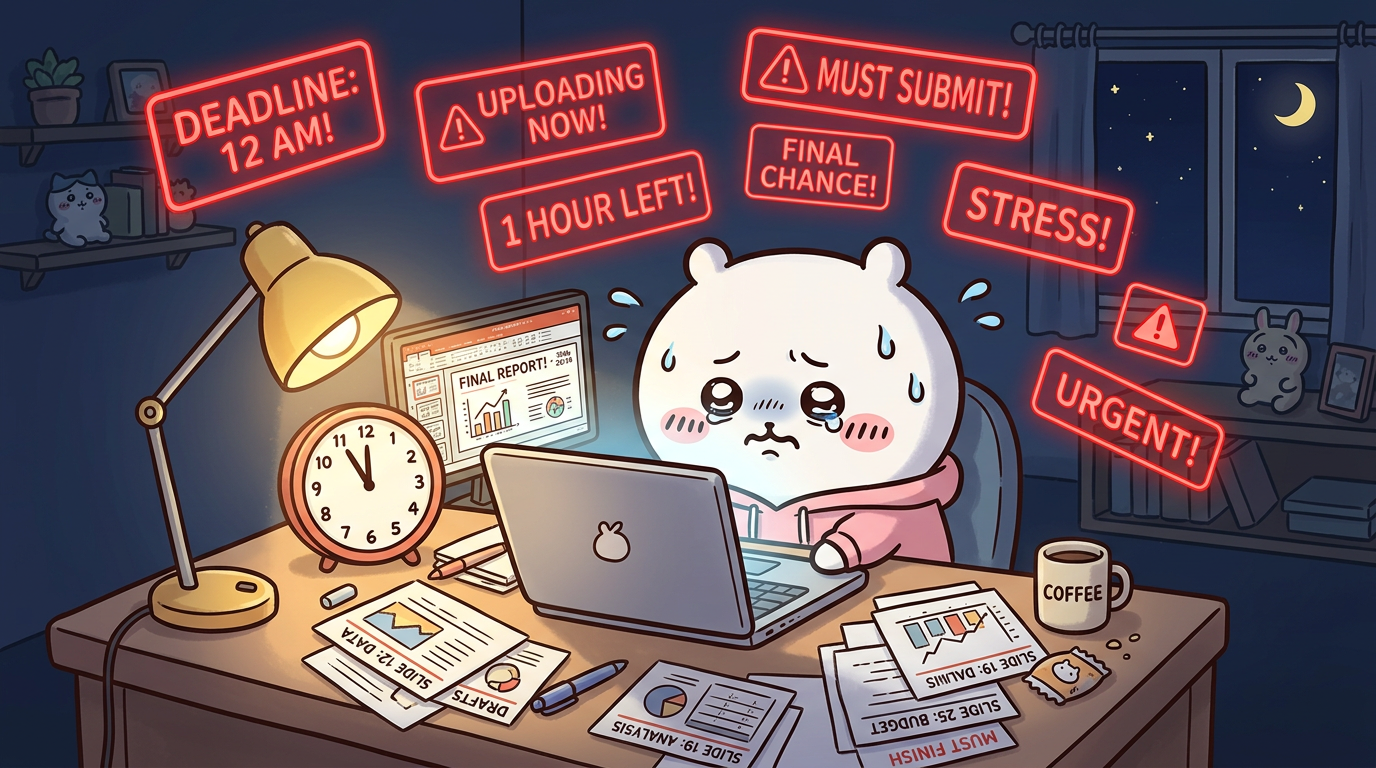
\includegraphics[width=\linewidth,keepaspectratio]{chiikawa-pain.png}\\[4pt]
      \footnotesize\textcolor{deepblue!60}{\textit{11 PM. Deadline at 9 AM.}}
    \end{column}
  \end{columns}
\end{frame}

%% ─────────────────────────────────────────────────────────────
%% Slide 3: Roadmap
%% ─────────────────────────────────────────────────────────────
\begin{frame}{全局路线图 Roadmap \sectag{Overview}}
  \vspace{4pt}
  \begin{center}
  \begin{tikzpicture}[node distance=1.0cm]
    \node[pbox,minimum width=2.6cm,text width=2.4cm] (n1) {\textbf{\S1}\\问题诊断\\{\tiny\EN{The Problem}}};
    \node[pbox,minimum width=2.6cm,text width=2.4cm,right=of n1] (n2) {\textbf{\S2}\\解法流程\\{\tiny\EN{The Pipeline}}};
    \node[pbox,minimum width=2.6cm,text width=2.4cm,right=of n2] (n3) {\textbf{\S3}\\技术规范\\{\tiny\EN{Tech Spec}}};
    \node[pbox,minimum width=2.6cm,text width=2.4cm,right=of n3] (n4) {\textbf{\S4}\\效果对比\\{\tiny\EN{Results}}};
    \draw[arr] (n1) -- (n2);
    \draw[arr] (n2) -- (n3);
    \draw[arr] (n3) -- (n4);
  \end{tikzpicture}
  \end{center}
  \vspace{8pt}
  \begin{columns}[c]
    \begin{column}{0.55\textwidth}
      \centering\small
      \textcolor{deepblue!50}{\rule{\textwidth}{0.4pt}}\\[4pt]
      \textit{"The best presentation tool is the one that}\\
      \textit{gets out of your way."}\\[2pt]
      \footnotesize\textcolor{deepblue!60}{— Design principle of this workflow}
    \end{column}
    \begin{column}{0.42\textwidth}
      \begin{alertblock}{\small 核心问题 Core Question}
        \footnotesize
        如何在不牺牲学术严谨性的前提下\\
        大幅提升汇报制作效率？\\[2pt]
        How to maximize presentation quality\\
        without sacrificing academic rigor?
      \end{alertblock}
    \end{column}
  \end{columns}
\end{frame}

%% ─────────────────────────────────────────────────────────────
%% Slide 4: S1 — The Problem
%% ─────────────────────────────────────────────────────────────
\begin{frame}{\S1\quad 三大 PPT 痛点 \sectag{The Problem}}
  \begin{columns}[T]
    \begin{column}{0.50\textwidth}
      \begin{block}{痛点 A：排版失控 \EN{Layout Chaos}}
        \footnotesize
        \begin{itemize}
          \item 字体跨平台乱版，Mac 好看 Windows 变形
          \item 手动调字号，一页一页点，效率极低
          \item 公式截图嵌入，放大后模糊失真
        \end{itemize}
      \end{block}
      \vspace{4pt}
      \begin{block}{痛点 B：内容分散 \EN{Content Fragmentation}}
        \footnotesize
        \begin{itemize}
          \item PPT、讲稿、参考文献分三个文件管理
          \item 修改一处，三个文件都要同步更新
          \item 版本混乱，不知道哪个是最新版
        \end{itemize}
      \end{block}
    \end{column}
    \begin{column}{0.46\textwidth}
      \begin{alertblock}{\small 痛点 C：质量无保证 \EN{No Quality Gate}}
        \footnotesize
        \textbf{传统流程}：做完就交，问题在讲台上才发现\\[4pt]
        常见问题：\\
        \quad $\bullet$ 溢出文字被裁掉\\
        \quad $\bullet$ TikZ/图表节点重叠\\
        \quad $\bullet$ 叙事逻辑跳跃，听众跟不上\\
        \quad $\bullet$ 讲稿与PPT对不上
      \end{alertblock}
      \vspace{4pt}
      \begin{exampleblock}{\small 数字说话 \EN{The Cost}}
        \footnotesize
        研究生平均每次汇报耗费：\\
        \textbf{4--6 小时}制作 PPT\\
        \textbf{另外 1--2 小时}写讲稿\\
        \alert{总计 5--8 小时，可以少很多}
      \end{exampleblock}
    \end{column}
  \end{columns}
\end{frame}

%% ─────────────────────────────────────────────────────────────
%% Slide 5: 8-Stage Pipeline
%% ─────────────────────────────────────────────────────────────
\begin{frame}[shrink=5]{\S2\quad 解法：8 阶段全自动流水线 \sectag{The Pipeline}}
  \begin{columns}[T]
    \begin{column}{0.50\textwidth}
      \vspace{2pt}
      \begin{center}
      \begin{tikzpicture}[node distance=0.28cm]
        \node[vbox,fill=deepblue!12] (s1) {\textbf{1} 素材摄入 Material Intake};
        \node[vbox,below=of s1] (s2) {\textbf{2} 脚手架搭建 Scaffold};
        \node[vbox,below=of s2] (s3) {\textbf{3} 内容生成 Content Generation};
        \node[vbox,below=of s3] (s4) {\textbf{4} AI 配图 Illustration};
        \node[vbox,fill=teal!10,below=of s4] (s5) {\textbf{5} 首次编译 First Compile};
        \node[vbox,fill=accent!8,below=of s5] (s6) {\textbf{6} 三重审查 Triple AI Review};
        \node[vbox,below=of s6] (s7) {\textbf{7} 讲稿生成 Script Generation};
        \node[vbox,fill=deepblue!18,below=of s7] (s8) {\textbf{8} 交付验证 Delivery Check};
        \foreach \a/\b in {s1/s2,s2/s3,s3/s4,s4/s5,s5/s6,s6/s7,s7/s8}
          \draw[arr] (\a) -- (\b);
      \end{tikzpicture}
      \end{center}
    \end{column}
    \begin{column}{0.46\textwidth}
      \centering
      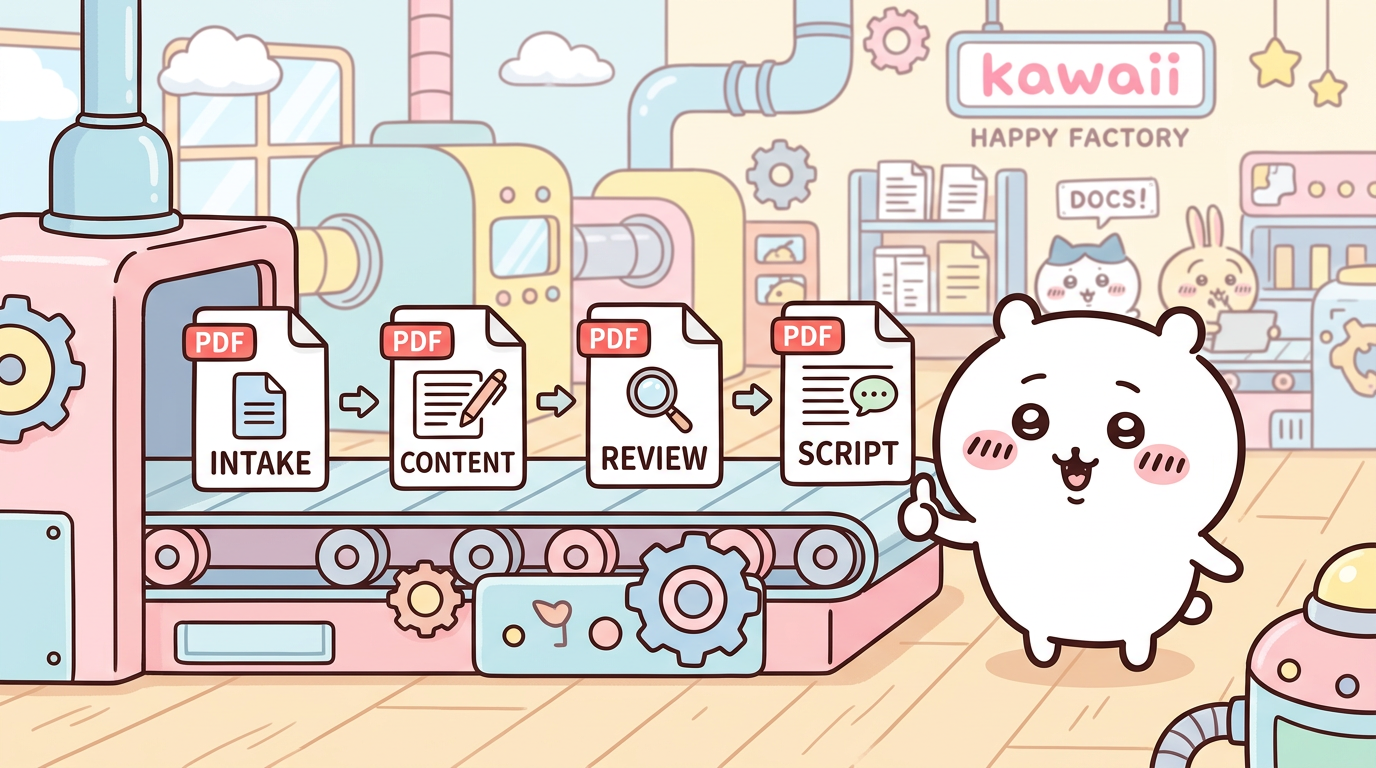
\includegraphics[width=0.92\linewidth,keepaspectratio]{chiikawa-pipeline.png}\\[6pt]
      \begin{alertblock}{\small 输出保证 \EN{Guaranteed Output}}
        \footnotesize
        每次运行必须交付：\\
        \quad \textcolor{teal}{$\checkmark$} \textbf{slides.pdf} — 幻灯片成品\\
        \quad \textcolor{teal}{$\checkmark$} \textbf{script.pdf} — 完整讲稿\\[2pt]
        所有 \texttt{.tex} 源文件可 \texttt{git} 追踪
      \end{alertblock}
    \end{column}
  \end{columns}
\end{frame}

%% ─────────────────────────────────────────────────────────────
%% Slide 6: Why not Office?
%% ─────────────────────────────────────────────────────────────
\begin{frame}{为什么不用 Office？ \EN{Why Not PowerPoint?} \sectag{Comparison}}
  \begin{columns}[T]
    \begin{column}{0.56\textwidth}
      \vspace{2pt}
      \footnotesize
      \begin{tabular}{>{\bfseries\color{deepblue}}p{2.0cm}
                       >{\color{teal!70!black}}p{2.2cm}
                       >{\color{accent}}p{2.2cm}}
        \toprule
        \textbf{维度} & \textbf{A Click} & \textbf{Office} \\
        \midrule\addlinespace
        排版精度 & XeLaTeX pt 精确 & 像素级手动调 \\[2pt]
        字体一致 & config.tex 一处 & 逐页点击改 \\[2pt]
        中英混排 & ctex 自动字距 & 手动调字号 \\[2pt]
        跨平台 & PDF 完全一致 & Win/Mac 差异 \\[2pt]
        图形质量 & TikZ 矢量 & 截图失真 \\[2pt]
        版本控制 & git diff .tex & .pptx 无差异 \\[2pt]
        讲稿同步 & 自动生成PDF & 另写文档 \\[2pt]
        智能审查 & AI 三重并行 & 人工单轮 \\
        \addlinespace\bottomrule
      \end{tabular}
    \end{column}
    \begin{column}{0.40\textwidth}
      \centering
      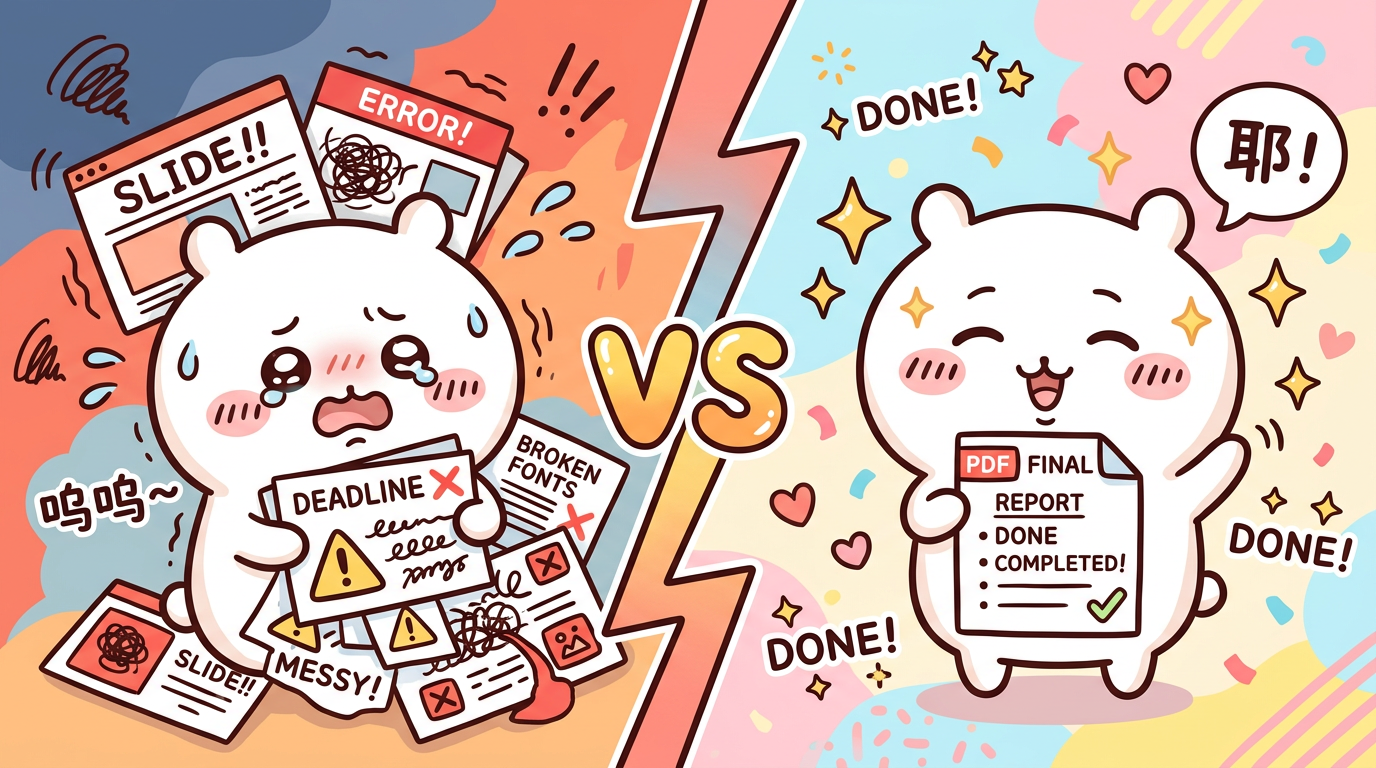
\includegraphics[width=\linewidth,keepaspectratio]{chiikawa-vs.png}\\[4pt]
      \begin{block}{\small 结论 Verdict}
        \footnotesize
        \alert{Office 的上限}是 A Click 的起点。\\[2pt]
        Office's ceiling is where\\
        A Click begins.
      \end{block}
    \end{column}
  \end{columns}
\end{frame}

%% ─────────────────────────────────────────────────────────────
%% Slide 7: 8 Advantages A–D
%% ─────────────────────────────────────────────────────────────
\begin{frame}[t,shrink=3]{8 大优点（上）\EN{Eight Advantages: A--D} \sectag{Features}}
  \begin{columns}[T]
    \begin{column}{0.48\textwidth}
      \begin{block}{\textcolor{deepblue}{\large\bfseries A}\quad 学术严谨性 \EN{Academic Rigor}}
        \footnotesize
        XeLaTeX pt 级精确排版，告别套模板\\
        PDF 跨平台完全一致，Office 无法保证
      \end{block}
      \vspace{6pt}
      \begin{block}{\textcolor{deepblue}{\large\bfseries C}\quad 完整流水线 \EN{End-to-End Pipeline}}
        \footnotesize
        8 阶段从摄入到交付，输出稳定可复现\\
        所有 .tex 源文件可 git 追踪回滚
      \end{block}
    \end{column}
    \begin{column}{0.48\textwidth}
      \begin{block}{\textcolor{deepblue}{\large\bfseries B}\quad 汇报自由度 \EN{Presentation Freedom}}
        \footnotesize
        叙事弧内置于工作流（Hook → Synthesis）\\
        TikZ 图形代码生成，中英双语无缝排版
      \end{block}
      \vspace{6pt}
      \begin{alertblock}{\textcolor{accent}{\large\bfseries D}\quad Plan 模式问需求 \EN{Requirements-First}}
        \footnotesize
        AI 不猜需求，先用5维问卷确认\\
        防止方向跑偏，节省 50\%+ 沟通成本
      \end{alertblock}
    \end{column}
  \end{columns}
  \vspace{4pt}
  \cluetag{A--D：从"做得出来"到"做得好"}
\end{frame}

%% ─────────────────────────────────────────────────────────────
%% Slide 8: 8 Advantages E–H
%% ─────────────────────────────────────────────────────────────
\begin{frame}[t,shrink=3]{8 大优点（下）\EN{Eight Advantages: E--H} \sectag{Features}}
  \begin{columns}[T]
    \begin{column}{0.48\textwidth}
      \begin{alertblock}{\textcolor{accent}{\large\bfseries E}\quad 三重 AI 审查 \EN{Triple AI Review}}
        \footnotesize
        slide-auditor · tikz-reviewer · pedagogy-reviewer\\
        并行审查，串行修复，最多 3 轮
      \end{alertblock}
      \vspace{6pt}
      \begin{alertblock}{\textcolor{accent}{\large\bfseries G}\quad AI 配图自动化 \EN{Auto Illustration}}
        \footnotesize
        摄入阶段规划配图，AI 生成后自动嵌入\\
        无需手动找图或处理分辨率
      \end{alertblock}
    \end{column}
    \begin{column}{0.48\textwidth}
      \begin{block}{\textcolor{deepblue}{\large\bfseries F}\quad 讲稿同步输出 \EN{Script Sync}}
        \footnotesize
        slides.pdf + script.pdf 永远同步交付\\
        \texttt{\textbackslash speakbox} 格式直接可朗读
      \end{block}
      \vspace{6pt}
      \begin{block}{\textcolor{deepblue}{\large\bfseries H}\quad 风格可配置 \EN{Style Configurable}}
        \footnotesize
        问卷选字体/配色，AI 写入 config.tex\\
        更换主题色只需修改 1 行
      \end{block}
    \end{column}
  \end{columns}
  \vspace{4pt}
  \cluetag{E--H：从"做得快"到"做得省心"}
\end{frame}

%% ─────────────────────────────────────────────────────────────
%% Slide 9: Plan Mode Intake
%% ─────────────────────────────────────────────────────────────
\begin{frame}{\S2\quad Plan 模式摄入 \EN{Plan Mode Intake} \sectag{How It Works}}
  \begin{columns}[T]
    \begin{column}{0.50\textwidth}
      \begin{exampleblock}{\small 触发词 Trigger Words}
        \footnotesize
        \texttt{帮我做个汇报}\\
        \texttt{Make me a presentation}\\
        \texttt{slides / PPT / beamer}
      \end{exampleblock}
      \vspace{4pt}
      \begin{block}{\small 5 个维度问卷 \EN{5-Dimension Questionnaire}}
        \footnotesize
        \begin{itemize}
          \item \textbf{内容} 主题 + 现有素材（PDF/DOCX）
          \item \textbf{格式} 页数 + 时长 + 是否双语
          \item \textbf{叙事} 故事线 / 直述 / 案例研究
          \item \textbf{输出} AI 配图？讲稿？
          \item \alert{\textbf{视觉}} 主色系 + 字体偏好 $\to$ config.tex
        \end{itemize}
      \end{block}
    \end{column}
    \begin{column}{0.46\textwidth}
      \begin{alertblock}{\small 视觉风格选项 \EN{Style Options}}
        \footnotesize
        \textbf{主色系：}\\
        \textcolor{deepblue}{$\blacksquare$} Deep Blue \quad
        \textcolor{teal}{$\blacksquare$} Forest Green \quad
        \textcolor{violet}{$\blacksquare$} Purple\\[4pt]
        \textbf{中文字体：}\\
        楷体 Kaiti SC \textbullet{} 黑体 PingFang \textbullet{} 宋体 Songti\\[4pt]
        \textbf{英文字体：}\\
        Times New Roman \textbullet{} Helvetica \textbullet{} Palatino
      \end{alertblock}
      \vspace{4pt}
      \begin{exampleblock}{\small 自动写入 Auto-Written}
        \footnotesize
        AI 将偏好写入 \texttt{config.tex}，\\
        全局生效，无需逐页调整。\\[2pt]
        AI writes your preferences to\\
        \texttt{config.tex} — one file, global effect.
      \end{exampleblock}
    \end{column}
  \end{columns}
\end{frame}

%% ─────────────────────────────────────────────────────────────
%% Slide 10: Content Generation
%% ─────────────────────────────────────────────────────────────
\begin{frame}{自动内容生成 \EN{Automated Content Generation} \sectag{Stage 3}}
  \begin{columns}[T]
    \begin{column}{0.50\textwidth}
      \begin{block}{输入 Input}
        \footnotesize
        \begin{itemize}
          \item 学术 PDF（章节内容）
          \item DOCX 提纲（结构参考）
          \item 用户笔记 / 口头描述
          \item config.tex（风格配置）
        \end{itemize}
      \end{block}
      \vspace{4pt}
      \begin{block}{生成内容 Generated}
        \footnotesize
        \begin{itemize}
          \item 双语幻灯片正文（逐页）
          \item TikZ 图形代码（流程图/DAG/三角图）
          \item 配图位置规划
          \item 叙事钩子与承转句
          \item 页脚/封面信息
        \end{itemize}
      \end{block}
    \end{column}
    \begin{column}{0.46\textwidth}
      \centering
      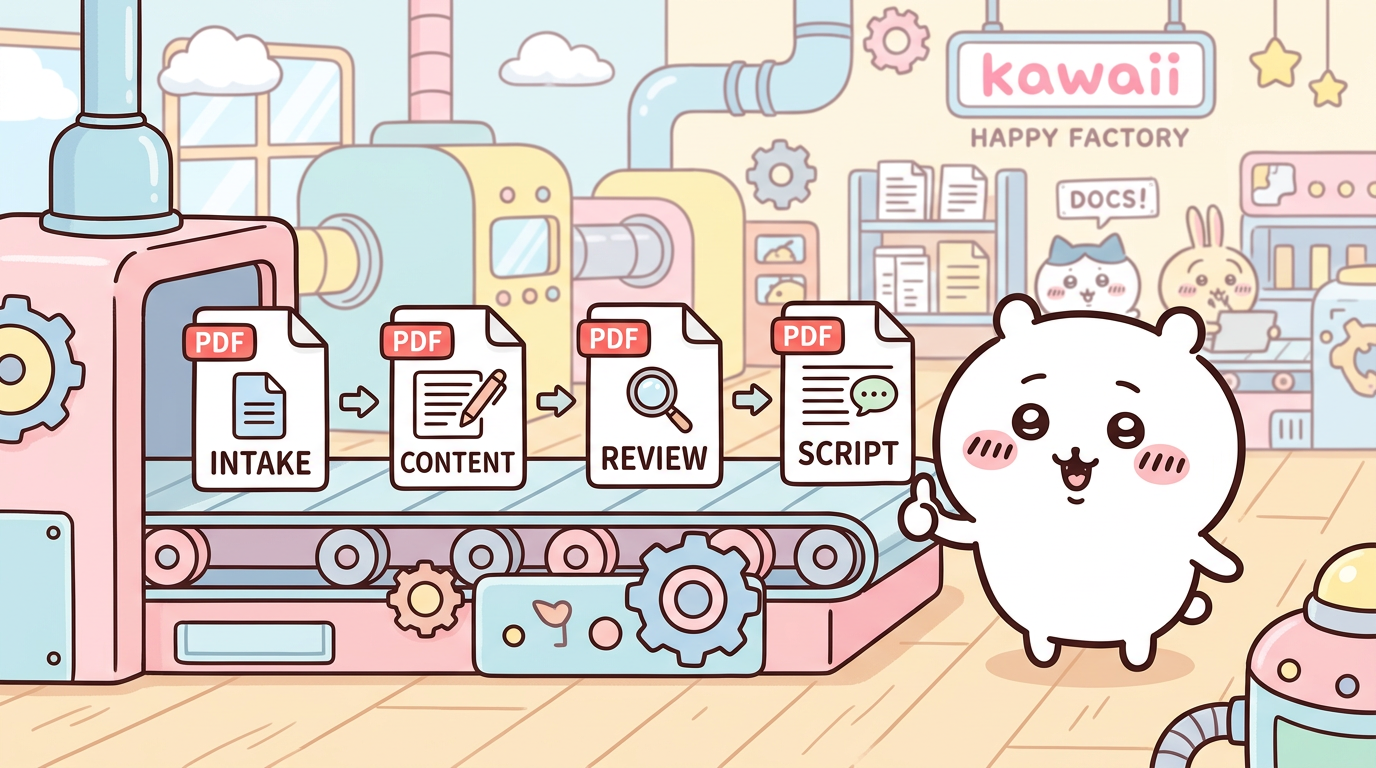
\includegraphics[width=\linewidth,keepaspectratio]{chiikawa-pipeline.png}\\[4pt]
      \begin{alertblock}{\small 关键技术约定}
        \footnotesize
        引号：Unicode 弯引号 \textcolor{gold}{``\,"} \\
        列内节点：\texttt{\textbackslash linewidth}\\
        溢出处理：\texttt{[shrink=8]}\\
        编译：XeLaTeX $\times$ 2
      \end{alertblock}
    \end{column}
  \end{columns}
\end{frame}

%% ─────────────────────────────────────────────────────────────
%% Slide 11: Triple AI Review
%% ─────────────────────────────────────────────────────────────
\begin{frame}{AI 三重质量审查 \EN{Triple AI Review} \sectag{Stage 6}}
  \begin{columns}[T]
    \begin{column}{0.52\textwidth}
      \vspace{6pt}
      \begin{center}
      \begin{tikzpicture}[scale=0.76]
        \node[trinode,fill=deepblue!12] (sa) at (0,2.5)
          {slide\\auditor};
        \node[trinode,fill=accent!12] (tr) at (-2.2,0)
          {tikz\\reviewer};
        \node[trinode,fill=teal!15] (pr) at (2.2,0)
          {pedagogy\\reviewer};
        \node[draw=gold,fill=gold!10,rounded corners=4pt,
              minimum width=2.2cm,minimum height=0.7cm,
              font=\footnotesize\bfseries] (fix) at (0,-1.4) {Fix Loop};
        \draw[arr,deepblue] (sa) -- (fix);
        \draw[arr,accent] (tr) -- (fix);
        \draw[arr,teal!70!black] (pr) -- (fix);
        \node[font=\tiny,text width=1.9cm,align=center,color=deepblue]
          at (0,3.5) {布局溢出\\字号检查\\图片引用};
        \node[font=\tiny,text width=1.9cm,align=center,color=accent]
          at (-3.5,0) {节点碰撞\\标签可读\\坐标检查};
        \node[font=\tiny,text width=1.9cm,align=center,color=teal!70!black]
          at (3.5,0) {叙事弧度\\术语一致\\节奏把控};
      \end{tikzpicture}
      \end{center}
    \end{column}
    \begin{column}{0.44\textwidth}
      \centering
      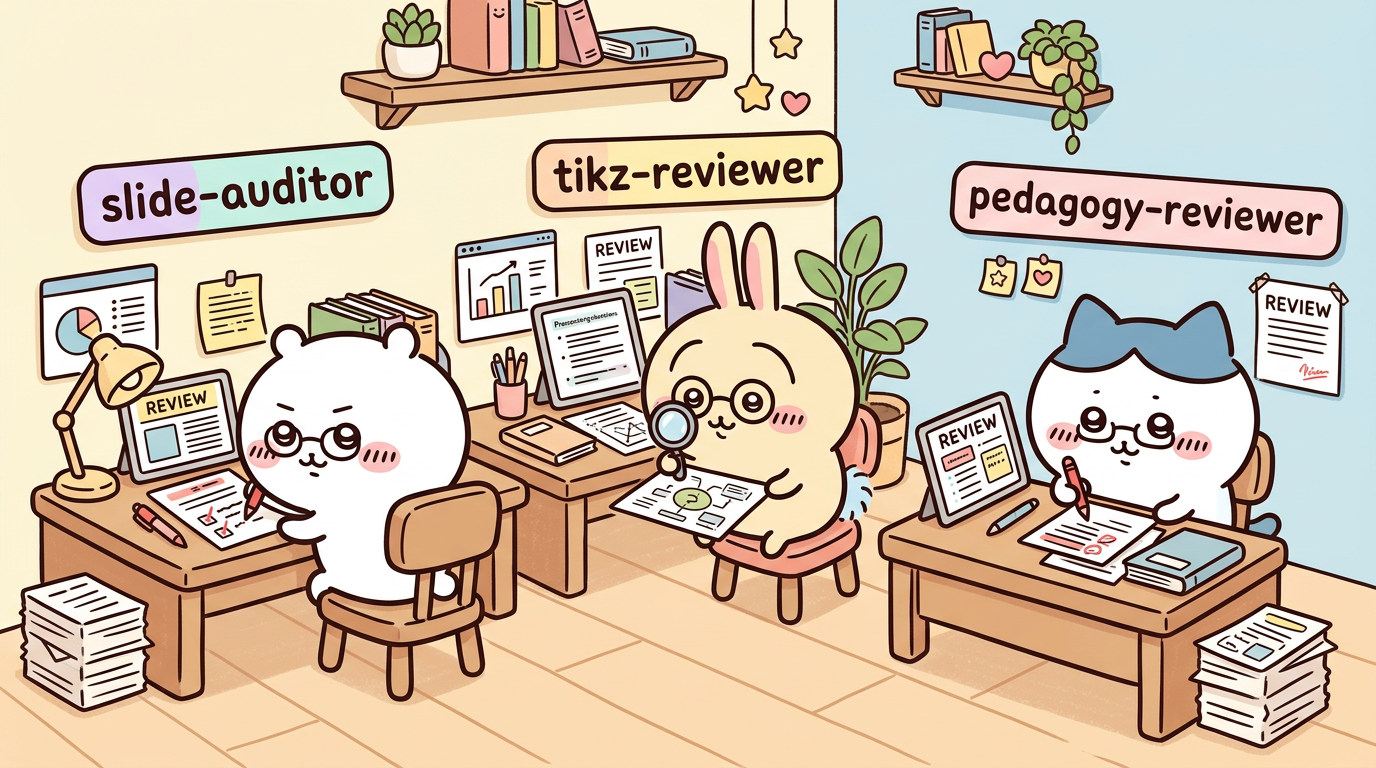
\includegraphics[width=\linewidth,keepaspectratio]{chiikawa-review.png}\\[6pt]
      \begin{block}{\small 审查规范}
        \footnotesize
        并行审查 → 串行修复\\
        最多 3 轮修复循环\\[2pt]
        Parallel review → serial fix\\
        Max 3 fix rounds
      \end{block}
    \end{column}
  \end{columns}
\end{frame}

%% ─────────────────────────────────────────────────────────────
%% Slide 12: Tech Spec — Fonts & Colors
%% ─────────────────────────────────────────────────────────────
\begin{frame}{\S3\quad 技术规范：字体与配色 \sectag{Tech Spec}}
  \begin{columns}[T]
    \begin{column}{0.50\textwidth}
      \vspace{4pt}
      \begin{center}
      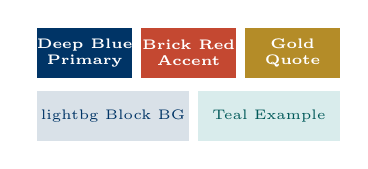
\begin{tikzpicture}[scale=0.80]
        \fill[deepblue] (0,2.8) rectangle (1.5,3.6);
        \node[white,font=\tiny\bfseries,align=center] at (0.75,3.2) {Deep Blue\\Primary};
        \fill[accent] (1.65,2.8) rectangle (3.15,3.6);
        \node[white,font=\tiny\bfseries,align=center] at (2.4,3.2) {Brick Red\\Accent};
        \fill[gold] (3.3,2.8) rectangle (4.8,3.6);
        \node[white,font=\tiny\bfseries,align=center] at (4.05,3.2) {Gold\\Quote};
        \fill[deepblue!15] (0,1.8) rectangle (2.4,2.6);
        \node[deepblue,font=\tiny,align=center] at (1.2,2.2) {lightbg Block BG};
        \fill[teal!15] (2.55,1.8) rectangle (4.8,2.6);
        \node[teal!70!black,font=\tiny,align=center] at (3.675,2.2) {Teal Example};
      \end{tikzpicture}
      \end{center}
      \vspace{4pt}
      \footnotesize
      \begin{tabular}{>{\bfseries\color{deepblue}}p{1.5cm} p{3.0cm}}
        \toprule
        Color & Usage 用途 \\
        \midrule
        deepblue & 标题/结构/主色 \\
        accent & 警告/强调 \\
        gold & 关键引言 \\
        teal & 示例块 \\
        \bottomrule
      \end{tabular}
    \end{column}
    \begin{column}{0.46\textwidth}
      \begin{block}{\small 字体矩阵 \EN{Font Matrix}}
        \footnotesize
        \begin{tabular}{ll}
          \toprule
          用途 & 字体 \\
          \midrule
          中文主体 & 楷体 Kaiti SC \\
          英文主体 & Times New Roman \\
          标题 & \textbf{加粗体} \\
          术语 & \textit{斜体标注} \\
          代码 & \texttt{等宽字体} \\
          \bottomrule
        \end{tabular}
      \end{block}
      \vspace{4pt}
      \begin{alertblock}{\small 风格参考}
        \footnotesize
        \textbf{Sant'Anna} — 配色体系\\
        \textbf{Andrews} — 信息层级\\
        \textbf{Tantau et al.} — Beamer 框架
      \end{alertblock}
    \end{column}
  \end{columns}
\end{frame}

%% ─────────────────────────────────────────────────────────────
%% Slide 13: config.tex
%% ─────────────────────────────────────────────────────────────
\begin{frame}[fragile]{用户配置：\texttt{config.tex} \sectag{User Config}}
  \begin{columns}[T]
    \begin{column}{0.54\textwidth}
      \begin{Verbatim}[fontsize=\tiny,frame=single,
                       rulecolor=\color{deepblue},
                       label={\footnotesize config.tex}]
%% CJK font
%% macOS: Kaiti SC | Win: KaiTi | Linux: AR PL UKai CN
\newcommand{\cjkfont}{Kaiti SC}

%% Latin font
\newcommand{\latinfont}{Times New Roman}

%% Primary color — Preset A (Academic Blue)
\definecolor{deepblue}{RGB}{0,52,102}
%% Preset B (Forest Green) — uncomment:
%% \definecolor{deepblue}{RGB}{0,80,60}
%% Preset C (Purple) — uncomment:
%% \definecolor{deepblue}{RGB}{60,20,100}

%% Footer text
\newcommand{\footleft}{Course · Topic}
      \end{Verbatim}
    \end{column}
    \begin{column}{0.42\textwidth}
      \begin{exampleblock}{\small 使用原则}
        \footnotesize
        \textbf{只修改 \texttt{config.tex}}\\
        不动 \texttt{slides-template.tex} 本体\\[4pt]
        Edit \texttt{config.tex} only.\\
        Never touch the template body.
      \end{exampleblock}
      \vspace{4pt}
      \begin{block}{\small 一处改，全局生效}
        \footnotesize
        \texttt{\textbackslash input\{config.tex\}} 在模板顶部\\
        字体、配色、页脚一次性切换\\[2pt]
        Single \texttt{\textbackslash input} at template top.\\
        Font, color, footer all switch at once.
      \end{block}
      \vspace{4pt}
      \begin{alertblock}{\small ppt-intake 自动生成}
        \footnotesize
        问卷回答后 AI 自动写入\\
        \texttt{config.tex}，无需手动编辑
      \end{alertblock}
    \end{column}
  \end{columns}
\end{frame}

%% ─────────────────────────────────────────────────────────────
%% Slide 14: Script Generation
%% ─────────────────────────────────────────────────────────────
\begin{frame}{讲稿生成机制 \EN{Script Generation} \sectag{Stage 7}}
  \begin{columns}[T]
    \begin{column}{0.50\textwidth}
      \begin{block}{\small \textbackslash speakbox — 口播内容}
        \footnotesize\color{deepblue}
        \textbf{🎤 口播内容}\\[2pt]
        各位好，今天我来分享的主题是…\\
        在我们开始之前，先讲一个故事。\\
        这个故事发生在某个深夜的实验室……
      \end{block}
      \vspace{6pt}
      \begin{exampleblock}{\small \textbackslash notebox — 舞台提示}
        \footnotesize\color{darkgray}
        \textbf{📋 舞台提示}\\[2pt]
        【PPT 提示：展示 Slide 2】\\
        【语速放慢，停顿 2 秒】\\
        【指向右边图片】
      \end{exampleblock}
    \end{column}
    \begin{column}{0.46\textwidth}
      \begin{alertblock}{\small 讲稿规范}
        \footnotesize
        \begin{itemize}
          \item 每页幻灯片对应一节
          \item \texttt{\textbackslash slidesec\{页码\}\{标题\}} 分节
          \item 口播内容与 PPT 内容严格对应
          \item 含计时提示（总时长控制）
          \item 叙事钩子在非核心部分自然嵌入
        \end{itemize}
      \end{alertblock}
      \vspace{4pt}
      \begin{block}{\small 输出格式}
        \footnotesize
        A4 纸 PDF，可直接打印\\
        \texttt{fancyhdr} 页眉：标题 + 讲稿人\\
        \texttt{geometry}：2cm 四边距\\
        字体与 slides 保持一致
      \end{block}
    \end{column}
  \end{columns}
\end{frame}

%% ─────────────────────────────────────────────────────────────
%% Slide 15: Before vs After
%% ─────────────────────────────────────────────────────────────
\begin{frame}[shrink=5]{\S4\quad 效果对比 \EN{Before vs After} \sectag{Results}}
  \vspace{4pt}
  \footnotesize
  \begin{tabular}{>{\bfseries\color{deepblue}}p{2.2cm}
                   >{\color{accent}}p{3.4cm}
                   >{\color{teal!70!black}}p{3.8cm}}
    \toprule
    \textbf{指标 Metric} &
    \textbf{传统方式 Before} &
    \textbf{A Click After} \\
    \midrule\addlinespace
    制作时间 & 5--8 小时，手动 & 20--40 分钟，自动化 \\[3pt]
    \multirow{2}{*}{排版质量} & 字体跑，截图模糊 &
      \multirow{2}{*}{XeLaTeX 矢量，完美} \\
    & 跨平台不一致 & \\[3pt]
    讲稿 & 另写，常与PPT脱节 & 自动生成，严格对应 \\[3pt]
    质量审查 & 上台前才发现问题 & 3 AI agents 把关 \\[3pt]
    可复现性 & 每次手动，差异大 & git 追踪，一键复现 \\[3pt]
    图形质量 & 截图，放大失真 & TikZ 矢量，任意缩放 \\[3pt]
    风格切换 & 全局修改，耗时 & config.tex 1 行搞定 \\
    \addlinespace\bottomrule
  \end{tabular}
\end{frame}

%% ─────────────────────────────────────────────────────────────
%% Slide 16: Delivery Spec
%% ─────────────────────────────────────────────────────────────
\begin{frame}{输出交付规范 \EN{Delivery Specification} \sectag{Stage 8}}
  \begin{columns}[T]
    \begin{column}{0.50\textwidth}
      \begin{block}{\small 必须交付 \EN{Must Deliver}}
        \footnotesize
        \begin{itemize}
          \item[\textcolor{teal}{$\checkmark$}] \textbf{slides.pdf} — 幻灯片成品
          \item[\textcolor{teal}{$\checkmark$}] \textbf{script.pdf} — 完整讲稿
          \item[\textcolor{teal}{$\checkmark$}] \textbf{slides.tex} — 源文件（可编辑）
          \item[\textcolor{teal}{$\checkmark$}] \textbf{config.tex} — 本次风格预设
          \item[\textcolor{teal}{$\checkmark$}] \textbf{images/} — 所有配图文件
        \end{itemize}
      \end{block}
      \vspace{4pt}
      \begin{exampleblock}{\small 质量门禁 \EN{Quality Gate}}
        \footnotesize
        交付前必须通过：\\
        \textcolor{teal}{$\checkmark$} PDF 可正常打开渲染\\
        \textcolor{teal}{$\checkmark$} 无文字溢出（Overfull box $<$ 10pt）\\
        \textcolor{teal}{$\checkmark$} 所有图片引用有效\\
        \textcolor{teal}{$\checkmark$} 讲稿页数 = 幻灯片页数
      \end{exampleblock}
    \end{column}
    \begin{column}{0.46\textwidth}
      \begin{alertblock}{\small 不得提前声明完成}
        \footnotesize
        \alert{不得在以下条件未满足时声明完成：}\\[4pt]
        $\times$ PDF 未能正常渲染\\
        $\times$ 主要审查问题未修复\\
        $\times$ 讲稿未生成\\
        $\times$ 用户要求的输出格式未达到\\[4pt]
        \textbf{Do not declare completion until}\\
        all deliverables are verified.
      \end{alertblock}
      \vspace{4pt}
      \begin{block}{\small 文件组织}
        \footnotesize
        \texttt{projects/presentations/}\\
        \quad\texttt{[slug]/slides.pdf}\\
        \quad\texttt{[slug]/script.pdf}\\
        \quad\texttt{[slug]/slides.tex}\\
        \quad\texttt{[slug]/images/}
      \end{block}
    \end{column}
  \end{columns}
\end{frame}

%% ─────────────────────────────────────────────────────────────
%% Slide 17: Design Inspiration & Credits
%% ─────────────────────────────────────────────────────────────
\begin{frame}{设计灵感与致谢 \EN{Inspiration \& Credits} \sectag{References}}
  \begin{columns}[T]
    \begin{column}{0.54\textwidth}
      \begin{block}{\small 排版风格参考 \EN{Typographic References}}
        \footnotesize
        \begin{itemize}
          \item \textbf{Pedro H.C. Sant'Anna}\\
            Vanderbilt / Microsoft Research\\
            {\tiny Beamer 配色体系与幻灯片节奏规范}\\
            {\tiny \textit{Beamer color palette \& slide rhythm conventions}}
          \vspace{2pt}
          \item \textbf{Isaiah Andrews}\\
            Harvard University\\
            {\tiny 学术汇报内容密度与信息层级}\\
            {\tiny \textit{Content density \& information hierarchy}}
          \vspace{2pt}
          \item \textbf{Till Tantau, J. Wright, V. Miletić}\\
            {\tiny \textit{The Beamer User Guide}}\\
            {\tiny 框架与宏设计 / Framework \& macro design}
        \end{itemize}
      \end{block}
    \end{column}
    \begin{column}{0.42\textwidth}
      \begin{exampleblock}{\small 技术栈 \EN{Tech Stack}}
        \footnotesize
        XeLaTeX + Beamer + ctex\\
        TikZ + booktabs + fontspec\\
        Cursor AI + ppt-pipeline skill\\
        slide-auditor + tikz-reviewer\\
        pedagogy-reviewer
      \end{exampleblock}
      \vspace{4pt}
      \begin{alertblock}{\small 开源许可 \EN{License}}
        \footnotesize
        MIT License\\
        \texttt{github.com/KyrieWong7/}\\
        \texttt{graduate-ppt-rescuer}\\[2pt]
        自由使用，保留署名\\
        Free to use with attribution
      \end{alertblock}
    \end{column}
  \end{columns}
\end{frame}

%% ─────────────────────────────────────────────────────────────
%% Slide 18: Ending
%% ─────────────────────────────────────────────────────────────
{
\setbeamercolor{background canvas}{bg=lightbg}
\begin{frame}[c]
  \begin{tikzpicture}[remember picture,overlay]
    \node[opacity=0.30,anchor=center] at (current page.center){%
      
\includegraphics[width=\paperwidth,height=\paperheight,
        keepaspectratio=false]{chiikawa-done.png}};
    \fill[lightbg,opacity=0.50]
      (current page.north west) rectangle (current page.south east);
  \end{tikzpicture}
  \begin{center}
    \vspace{8pt}
    {\Large\bfseries\textcolor{deepblue}{A Click is All You Need}}\\[8pt]
    \textcolor{gold}{\rule{0.618\textwidth}{0.8pt}}\\[10pt]
    {\large\textcolor{gold}{\textbf{\textit{%
      "One sentence. One click. Two PDFs."}}}}\\[12pt]
    \footnotesize\textcolor{deepblue!70}{%
      slides.pdf \quad\textbullet\quad script.pdf \quad\textbullet\quad git push}\\[8pt]
    \footnotesize\textcolor{deepblue!60}{%
      \texttt{github.com/KyrieWong7/graduate-ppt-rescuer}}\\[6pt]
    \scriptsize\textcolor{deepblue!50}{%
      Generated by the pipeline it describes.}
  \end{center}
\end{frame}
}

\end{document}
